\documentclass[12pt,a4paper]{article}
\usepackage[utf8x]{inputenc}
\usepackage{ucs}
\usepackage{amsmath}
\usepackage{amsfonts}
\usepackage{amssymb}
\usepackage{graphicx}
\usepackage{listings}
\usepackage[left=2cm,right=2cm,top=2cm,bottom=2cm]{geometry}

\usepackage{natbib}
\bibpunct{[}{]}{,}{n}{}{;}

\usepackage[pdftex,pagebackref]{hyperref}
    \usepackage{natbib}
    \hypersetup{colorlinks,linktocpage=true}
\renewcommand{\backrefpagesname}{ \protect\\  \textit{Cited on
page(s):}~}
\renewcommand{\backref}{\backrefpagesname}

\author{Gergely Imreh}
\title{Quadruple coil drive circuits}
\date{2013-03-21, v1}
\begin{document}
\maketitle

The coils in the experimental system creating the quadruple magnetic field have much higher requirements than the usual MOT experiments. Have to create very large magnetic field gradients, and have to ramp, switch on/off in a short time.

\tableofcontents

\section{Requirements}

Being able to supply up to 400A. Ramping between the 100\% and ~20\% in a few seconds. Switching on in ~ millisecond, and off in few hundred microsecond.


\section{Semiconductor selection}

\subsection{MOSFET}

\subsection{IGBT}

\begin{figure}[ht!]
\centering
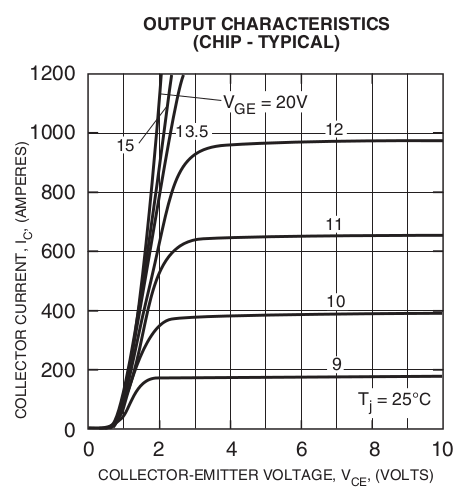
\includegraphics[width=90mm]{CM600DY-24S_I_V.png}
\caption{I-V curve for CM600DY-24S}
\label{fig:cm600dy}
\end{figure}


\subsection{IGBT vs MOSFET}

\begin{figure}[ht!]
\centering
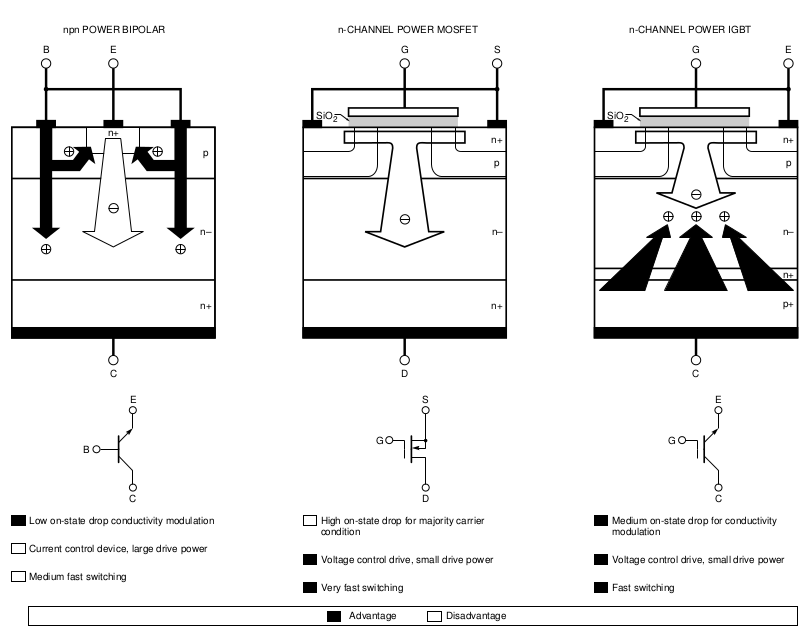
\includegraphics[width=150mm]{comparison1.png}
\caption{Comparison of BJT, MOSFET, and IGBT, from \cite{MitsubishiIGBT}.}
\label{fig:comparison1}
\end{figure}

Just switching: use high $V_{GE}$, constant current, and be in the edge of the $I-V$ curve.

Feedback and control: use constant voltage, be in the saturation region, and feed back to the $V_{GE}$. Maybe that idea doesn't work, based on \citep{Bortis2008}.

Comparison \cite{Blake}

\section{Complete circuit}

\begin{figure}[ht!]
\centering
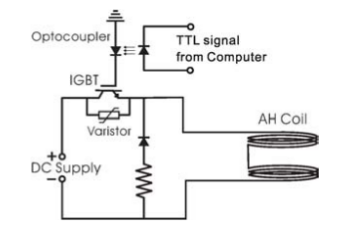
\includegraphics[width=100mm]{Yum2012_circuit.png}
\caption{From \cite{Yum2012}}
\label{fig:yum2012circuit}
\end{figure}


From \cite{Yum2012}: IGBT is Powerex (Mitsubishi) PM800HSA120\footnote{PM800HSA120 product page: \url{http://www.pwrx.com/Product/PM800HSA120}}, varistor TNR20E391K\footnote{TNR20E391K simple specs: \url{http://www.pucko-elektronik.com/download/nwar/tnre.pdf}} (x5 parallel), diode MDF25A40\footnote{MDF25A40 product page: \url{http://www.galco.com/buy/Sanrex-Sansha-Electric-Manufacturing/MDF250A40}}, resistor Alcol NHS250 1 Ohm (x3 parallel).


Simulation


NIST: 1) MOSFET FB180SA10, varistor S20K25, other MOSFET STE250NS10 2) Powerex CM600HA-24A (switching between dummy coil and real coil), Hall probe FW Bell


GMR magnetic field sensor (NVE)

Precision current resistor TGHG series  (Ohmite) (doesn't work directly, because it has a 50A limit)

Timing: don't want multiple of them in the same time, it becomes really difficult


Resistance budget is tricky - cable, contacts, coil, IGBT... likely push the system to its limits

Agilent 6690A

Advantage disadvantage, and I-V curves \cite{Sattar} (current tail, dead time between switching, otherwise very similar)

\bibliographystyle{unsrtnat}
\bibliography{quadcoil}

\end{document}